\documentclass[11pt]{article}
\usepackage[utf8]{inputenc}
\usepackage{graphicx}
\usepackage{enumitem}
%\setlist{nosep}
\usepackage{subcaption}
\usepackage{booktabs}
\usepackage{microtype}      % microtypography
\usepackage{textcomp}
\usepackage{gensymb}
\usepackage{caption}
\usepackage{xcolor}
\usepackage{longtable}
\usepackage{setspace}

\usepackage{amsmath,amssymb,amsthm}
\usepackage{parskip}
\usepackage{float}
\usepackage{multirow}
\usepackage[normalem]{ulem}
\usepackage{comment}
\usepackage[left=1.5in, right=1in, top=1in, bottom=1in]{geometry}
\renewcommand{\familydefault}{\sfdefault}
\usepackage{appendix}

\usepackage{hyperref}
\usepackage{url}

\hypersetup{
	colorlinks   = true,
	citecolor    = black!60
}

\captionsetup{
	format = plain,
	textfont = small,
	labelfont = {normalsize,bf,color=gray},
	figurename = FIGURE,
	tablename = TABLE,
	labelsep = quad,
	singlelinecheck=false
}

\usepackage[sort&compress]{natbib}
\renewcommand{\bibfont}{\footnotesize}
\bibliographystyle{./bst/plant_physiology_url}

\linespread{1.5}

\graphicspath{ {./figs/} }

\usepackage[mathlines]{lineno}
\linenumbers
\renewcommand\linenumberfont{\normalfont\scriptsize}
\setlength\linenumbersep{3ex}

%\renewcommand{\familydefault}{\sfdefault}
\renewcommand{\appendixpagename}{Supplementary data}
\newcommand{\review}[1]{\textcolor{blue}{#1}}

\begin{document}
	
	{\setlength{\parindent}{0cm}
		{\Large
			\textbf{%
				Land Grant collaborative networks for plant science research
			}
		}
		
		Roberto Herrera\textsuperscript{1,2,\textdagger}, 
		Sophia Knehans\textsuperscript{1,\textdagger}, 
		David M. Braun\textsuperscript{3,4}, 
		Erik J. Am\'ezquita\textsuperscript{1,3,\textdaggerdbl}
		
		%\vspace{1em}
		{\footnotesize
			\textsuperscript{1}Department of Mathematics, 
			\textsuperscript{2}Department of Electrical Engineering and Computer Science, 
			\textsuperscript{3}Division of Plant Sciences \& Technology,
			\textsuperscript{4}Division of Biological Sciences,
			University of Missouri, Columbia, MO 65211, USA
			
		}
		
		%\vspace{1em}
		
		%\vspace{1em}
		Keywords: 
		
		\vfill
		\textsuperscript{\textdagger}Contributed equally to this work
		
		\textsuperscript{\textdaggerdbl}
		To whom correspondence should be addressed:
		
		Erik J. Am\'ezquita
		\vspace{-1em}
		
		371h Bond Life Sciences Center, Columbia, MO 65211
		\vspace{-1em}
		
		\url{eah4d@missouri.edu}
	}
	\pagebreak
	
	\begin{abstract}
		Write abstract
	\end{abstract}
	
	\section{Introduction}
	
	Motivation. Big picture. Literature review. 
	
	Here, we study\ldots
	
	\section{Materials and methods}
	
	Data collected from Dimensions. Publications from the 51 land grant institutions listed in Y. Years considered. Information discarded. Caveats. \citep{Smith2018, Voo2012}
	
	\section{Results}
	
	A placeholder figure
	
	\begin{figure}[h!]
		\centering
		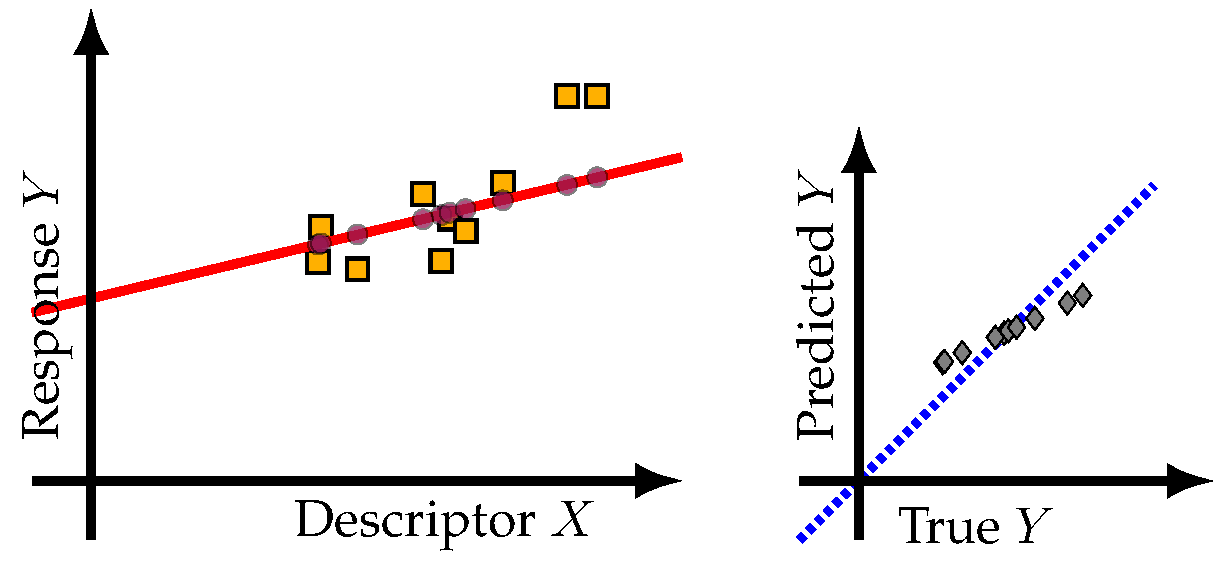
\includegraphics[width=0.9\textwidth]{placeholder.pdf}
		\caption{%
			\textbf{Title and one sentence description}. More detailed caption.}
	\end{figure}
	
	
	\section{Discussion}
	
	\section*{Acknowledgments}
	
	\section*{Author contributions}
	
	\section*{Software and data availability}
	
	\section*{Conflict of interests}
	
	None declared
	
	\section*{Figure and table captions}
	
	\section*{Supplementary figure and table captions}
	
	\bibliography{biblio}
	
	\newpage
	
	\appendix
	\appendixpage
	
	\setcounter{figure}{0}
	\makeatletter
	\renewcommand{\thefigure}{S\@arabic\c@figure}
	\makeatother
	
\end{document}